\chapter{The KryBall Optimiser}
\label{chap:method}

In this chapter, we present our method, the Krylov optimiser. We first introduce the concept of the Saddle-Free-Newton that our method builds upon on in \cref{sec:saddle_free_newton}. We then present our algorithm, which includes core components such as Krylov subspace construction, the use of the Saddle-Free-Newton, and a trust-region framework. This is detailed in \cref{sec:kryball_optimisation_algorithm}. We then present the main algorithm in \cref{sec:main_algorithm}.

\section{Saddle-Free-Newton}
\label{sec:saddle_free_newton}

We build upon a key work in optimisation, the \textit{Saddle-Free-Newton} (SFN) method. Recall in \cref{sec:second_order_methods}, we showed that the pure Newton method can be attracted to saddle points due to optimising in a non-convex setting. To address this problem, the SFN method was proposed \citep{dauphin2014sfn}. The SFN is essentially a regularised Newton method, similar to that of Damped Newton methods we saw in \cref{ssec:newton_methods}. However, instead of applying step-size or regularisation damping, the SFN method instead applies the $|\cdot|$ (abs) function onto the \textit{eigenvalues} of the Hessian. This results in an adjusted Hessian which is \textit{guaranteed} to be positive semi-definite, and thus avoids being attracted to saddle points. 

\begin{definition}[Saddle-Free-Newton Step]
    Given a Hessian $H$ and a gradient $g$ evaluated at our current parameters $\theta$, we define the Saddle-Free-Newton step $\Delta \theta_{SFN}$ as:
    \begin{align}
        H &= V \Lambda V^T \\
        H^{SFN} &= V |\Lambda| V^T \\
        \Delta \theta_{SFN} &= -(H^{SFN})^{-1} g,
    \end{align}
    where $\Lambda$ is the diagonal matrix of eigenvalues, and $|\cdot|$ is the element-wise absolute value applied to each element of $\Lambda$.
\end{definition}
We use the notation $\| H \|$ and $H^{SFN}$ interchangeably to refer to the reconstructed Hessian that is now guaranteed to be positive semi-definite. We illustrate this change in \cref{fig:guaranteed_pos_def}.

\begin{figure}
    \centering
    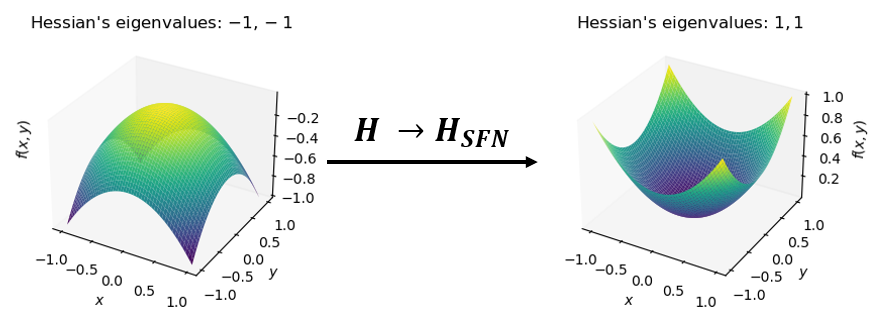
\includegraphics[width=0.8\linewidth]{figures/4method/method_diag_1.png}
    \caption{The crux of the SFN step: A non positive-semi-definite $H$ is now be guaranteed to be positive semi-definite as we manipulate the curvature information by applying $|\cdot|$ to the eigenvalues $\Lambda$ of $H$ to form $H^{SFN}$.}
    \label{fig:guaranteed_pos_def}
\end{figure}

As an example, consider once again our 2D horse saddle function from \cref{ssec:second_order_methods}. Recall we split the problem into two cases to optimise: $g(x) = x^2$ and $h(y) = -y^2$. We computed that $H_g = \nabla^2 g(x) = 2$ in the $x$-direction and $H_h = \nabla^2 h(y) = -2$ in the $y$-direction given our starting iterates $(x_0, y_0) = (1.5, 1.5)$. Our problem with Newton's method was that $H_h$ had a negative eigenvalue, which made our Hessian indefinite and thus in the y-direction, we moved towards the local maximum instead. Now, we consider the SFN step and it's behaviour.
\begin{itemize}
    \item In the $x$-direction, we have $H_g = 2$. Applying $|\cdot|$ to the eigenvalues, we get $H^{SFN} = 2$. This is the same as the Newton step, which behaves correctly for this case, so $x_1 = 0$.
    \item In the $y$-direction, we have $H_h = -2$. Applying $|\cdot|$ to the eigenvalues, we get $H^{SFN} = 2$. Now, we have that
    \begin{align}
        y_1 = y_0 + \Delta y = y_0 - (H^{SFN})^{-1} \nabla h(y_0) = y_0 - \frac{1}{2} \cdot (-2 y_0) = y_0 + y_0 = 2y_0.
    \end{align}
    Given we have $y_0 = 1.5$, our next iterate is $y_1 = 2 \cdot 1.5 = 3$. This is the correct behaviour, and we have successfully moved \textit{away} from the saddle point and follow the negative gradient direction.
\end{itemize}
As a result, our next set of iterates $(x_1, y_1) = (0, 3)$ now evaluates to $f(0, 3) = -9$. Thus, we have moved away from the saddle point. Subsequently applying more SFN steps will optimise $f$ more until we diverge, since the function is unbounded. We illustrate our discussion in \cref{fig:newton_attract}.

\begin{figure}[h]
    \begin{subfigure}[b]{0.33\linewidth}
        \centering
        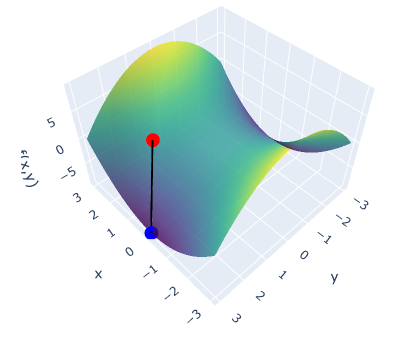
\includegraphics[width=\linewidth]{figures/4method/sfn_2d.png}
        \caption{The SFN step on the 2D horse saddle function.}
        \label{fig:sfn_2d}
    \end{subfigure}
    \hfill
    \begin{subfigure}[b]{0.32\linewidth}
        \centering
        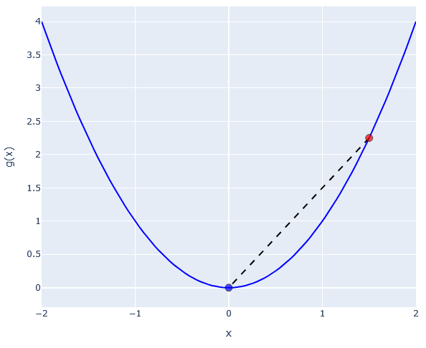
\includegraphics[width=\linewidth, height=100px]{figures/4method/sfn_x.png}
        \caption{The SFN step on the $x$-axis component}
        \label{fig:sfn_x}
    \end{subfigure}
    \hfill
    \begin{subfigure}[b]{0.33\linewidth}
        \centering
        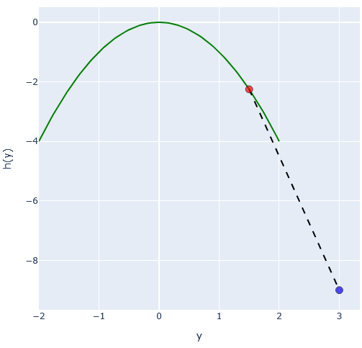
\includegraphics[width=\linewidth, height=100px]{figures/4method/sfn_y.png}
        \caption{The SFN step on the $y$-axis component,}
        \label{fig:sfn_y}
    \end{subfigure}
    \caption{SFN on the classic 2D horse saddle function. Unlike the Newton step, the SFN step is not attracted to the saddle points. 
    Given a starting point $(1.5, 1.5)$ in red, the SFN step is able to move away from the saddle point and decrease the objective function. For both the $x$-axis and $y$-axis components, the SFN step is able to move in the correct direction.}
    \label{fig:sfn_example}
\end{figure}

However, while the SFN method addresses the issue, the core limitation is still the computational intractability. To compute the SFN, we must do an eigendecomposition of the Hessian, apply our abs function, reconstruct it, and then take the inverse. This sequence of steps is infeasible for deep learning.  

\section{The KryBall Optimisation Algorithm}
\label{sec:kryball_optimisation_algorithm}
This raises the question: how can we compute the SFN step efficiently, especially given the proliferation of saddle points? We thus introduce KryBall, a method that extends the SFN method and uses its advantages while being computationally tractable for deep learning. KryBall is a second-order method that uses Krylov subspaces, the SFN step, and a trust-region framework. At it's core, KryBall consists of two main components: 
\begin{itemize}
    \item \textbf{SFN Computation}: The efficient computation of the SFN step direction.
    \item \textbf{Trust-Region Framework}: The integration of the SFN step and other useful components into a generalised trust-region framework.
\end{itemize}
In this section, we detail these two core components. We first discuss how to compute the SFN step direction in \cref{sec:computation_of_the_saddle_free_newton}. We then present how we integrate this into a trust-region framework in \cref{sec:n_dimensional_subspace_optimisation}. Finally, we present our main algorithm in \cref{sec:main_algorithm}.

\subsection{Computation of the Saddle-Free-Newton}
\label{sec:computation_of_the_saddle_free_newton}

We introduced Krylov subspaces in \cref{ssec:krylov_subspaces}. We now use them to their best ability in our method. Instead of computing and storing the full Hessian, we can generate a Krylov subspace with the Hessian $H$ and the gradient $g$. This gives us,
\begin{align}
    \mathcal{K}_{M}(H, g) = \text{span} \{g, H g, H^2 g, \ldots, H^{M-1} g \}, 
\end{align}
which allows us to approximate the action of the Hessian. Recall that the Arnoldi iteration not only generates an orthonormal basis $Q_M$ for $\mathcal{K}_{M}(H, g)$, but also the coefficient matrix $H_M$. We know that this is a projection of the original space that we work in. That is, we now have the following relationship,
\begin{align}
    Q_M^T H Q_M = H_M,
\end{align}
where $H_M$ is the \textit{projected Hessian}. Thus, we now have a low-dimensional approximation of our original space $H$ through the projected Hessian $H_M$. We then use this to compute the SFN step direction.
\begin{align}
    H_M = V_M \Lambda_M V_M^T \\
    H_M^{SFN} = V_M |\Lambda_M| V_M^T \\
    \Delta \theta_{SFN} = -(H_M^{SFN})^{-1} q_0, \quad q_0 = \frac{g}{\| g \|},
\end{align}
The gradient projected into this subspace is $g_M = Q_M^T g_t$. Since $q_0 = g_t/\|g_t\|_2$, $g_M$ is simply $\|g_t\|_2 e_1$, where $e_1$ is the first standard basis vector in $\mathbb{R}^M$. Note that we assume $H_M$ is symmetric here even though we have not explicitly assumed this in our Arnoldi iteration. For this case, we do not use the last row of $H_M$ and thus our $H_M$ goes from being a $M+1 \times M+1$ matrix to a $M \times M$ matrix. We do this since we only need the first $M$ eigenvalues of $H_M$ to compute the SFN step. After we compute the SFN step, we then project it back into the original space as follows,
\begin{align}
    \Delta \theta_{SFN} = Q_M \Delta \theta_{SFN}.
\end{align}
We now have our SFN direction that we can use to optimise our model. In KryBall, we offer an almost one to one implementation of this. However, we make one slight modification and add a clipping parameter $\epsilon$ for numerical stability. This ensures that the step direction and norm are not too large, and thus we do not diverge from the original space. We perform the clipping after we apply the abs operator to the eigenvalues. Formally, we write this as,
\begin{align}
    H_M^{SFN} = V_M \text{clip}(|\Lambda_M|, \epsilon) V_M^T \\
    \Delta \theta_{SFN} = -(H_M^{SFN})^{-1} q_0,
\end{align}
where the clipping function $\text{clip}(x, \epsilon)$ clips any eigenvalues of $H_M$ that are less than $\epsilon$ to $\epsilon$.

\subsection{N-Dimensional Subspace Optimisation}
\label{sec:n_dimensional_subspace_optimisation}

Having computed the SFN direction $\Delta \theta_{SFN}$, we now integrate into a robust step selection procedure using $N$-dimensional subspace optimisation. We introduced briefly 2D subspace optimisation in \cref{ssec:trust_region_methods}. The general principles are extended to the $N$-dimensional case. 

We define a search subspace $\mathcal{S}_k$ as a $k$-dimensional subspace that is spanned by a set of $k$ informative direction vectors. These vectors are chosen to capture both first-order and approximated second-order information about the loss landscape. Typically, the basis vectors for $\mathcal{S}_k$ include:
\begin{itemize}
    \item The normalised current gradient: $g_t / \|g_t\|_2$.
    \item The normalised SFN direction: $\Delta \theta_{SFN} / \|\Delta \theta_{SFN}\|_2$, as computed in \cref{sec:computation_of_the_saddle_free_newton}.
    \item The normalised momentum vector: $z_t / \|z_t\|_2$, which aggregates information from past gradients.
\end{itemize}
Let $X_t = [x_1, x_2, \ldots, x_k]$ be the matrix whose columns are these $k$ orthonormalised basis vectors. Any potential step $p_t$ from the current iterate $\theta_t$ is therefore restricted to this subspace, meaning $p_t = X_t \alpha$ for some coefficient vector $\alpha \in \mathbb{R}^k$.

The core of the trust-region method is to minimise a quadratic model $m_t(p)$ of the loss function $L(\theta_t + p)$ within this subspace $\mathcal{S}_k$, subject to the constraint that the step $p_t$ remains within a trust region of radius $\Delta_t$. The quadratic model is given by:
\begin{align}
    m_t(p) = L(\theta_t) + g_t^T p + \frac{1}{2} p^T H_t p.
\end{align}
Substituting $p = X_t \alpha$, the subproblem becomes finding $\alpha^*$ that solves:
\begin{align}
    \min_{\alpha \in \mathbb{R}^k} & \quad (X_t^T g_t)^T \alpha + \frac{1}{2} \alpha^T (X_t^T H_t X_t) \alpha \label{eq:tr_subspace_objective} \\
    \text{subject to} & \quad \|X_t \alpha\|_2^2 \leq \Delta_t^2. \label{eq:tr_subspace_constraint}
\end{align}
Let $b_k = X_t^T g_t$ be the projection of the gradient onto the subspace directions, and $A_k = X_t^T H_t X_t$ be the projection of the Hessian onto the subspace. We can compute $A_k$ efficiently using HVPs $H_t x_i$ for each basis vector $x_i$ in $X_t$. The objective function in \cref{eq:tr_subspace_objective} then simplifies to $b_k^T \alpha + \frac{1}{2} \alpha^T A_k \alpha$.

This $k$-dimensional trust-region subproblem is solved to find the optimal coefficients $\alpha^*$. The resulting step in the full parameter space is $p_t^* = X_t \alpha^*$. We then follow suite with the standard trust-region algorithm and update our radius based on the reduction ratio. If we cannot ensure sufficient reduction, we reject the step and adapt our radius accordingly and try again. This ensures that the algorithm adapts to the reliability of the quadratic model, promoting stable and efficient convergence.


\section{Main Algorithm}
\label{sec:main_algorithm}

We now bring together the previously described components: the efficient computation of the SFN direction via Krylov subspaces, and its integration into an $N$-dimensional subspace optimisation using a trust-region framework. We present the complete KryBall optimisation algorithm in \cref{alg:kryball_algorithm}.

\begin{algorithm}[h] % H for "here definitely" placement
    \DontPrintSemicolon
    \KwIn{Initial parameters $\theta_0$, objective function $L(\theta)$, Krylov dimension $M$, trust-region parameters (initial radius $\Delta_0$, max radius $\Delta_{\mathit{max}}$, adaptation rules $\eta_1, \eta_2$), Krylov refresh rate $r_{\mathit{refresh}}$, momentum factor $\beta$}
    \KwOut{Optimised parameters $\theta^*$}
    
    Initialise $\theta \leftarrow \theta_0$, trust-region radius $\Delta \leftarrow \Delta_0$\;
    Initialise momentum vector $z \leftarrow 0$\;
    
    \For{$t=0, 1, 2, \ldots$ until convergence}{
        Compute current gradient $g_t = \nabla L(\theta_t)$\;
        \If{$t \pmod{r_{\mathit{refresh}}} == 0$}{
            Construct orthonormal $Q_M$ and $H_M$ from the Arnoldi iteration for $\mathcal{K}_M(H_t, g_t)$\;
            Compute and normalise $\Delta \theta_{SFN}$\;
        }
        
        Define search subspace directions $X_S = [g_t / \|g_t\|_2, z_t / \|z_t\|_2]$\;
        \If{$t \pmod{r_{\mathit{refresh}}} == 0$}{
            Add SFN direction $\Delta \theta_{SFN}$ to $X_S$
        }
        \Else{
            Add basis vectors of $Q_M$ to $X_S$
        }
        Project gradient $b_k = X_t^T g_t$\;
        Project Hessian $A_k = X_t^T H_t X_t$\;
        
        Solve the trust-region subproblem to find $\alpha^*$\;
        Compute candidate step $p_t = X_t \alpha^*$\;
        
        Compute the reduction $\rho_t$\;
        Accept or reject the step based on $\rho_t$ and $\|p_t\|$\;
        Update $\Delta_{t+1}$ based on $\rho_t$, $\|p_t\|$, and $\Delta_{\mathit{max}}$\;
        Update momentum vector $z_{t+1} \leftarrow \beta  z_t + g_{t+1}$\;
        $\theta \leftarrow \theta_{t+1}$, $\Delta \leftarrow \Delta_{t+1}$\;
    }
    \Return{$\theta$}\;
    \caption{The KryBall Optimisation Algorithm}
    \label{alg:kryball_algorithm}
\end{algorithm}

The algorithm iteratively builds a low-dimensional quadratic model of the objective function. It leverages curvature information approximated via the SFN direction computed within a Krylov subspace. An optimal step is then determined within this subspace using the trust-region framework, which adaptively adjusts the step size to ensure reliable progress.

Note that we have a refresh parameter $r_{\mathit{refresh}}$ which controls how often we update our Krylov basis. This is primarily for efficiency reasons, as it is expensive to compute the Arnoldi iteration every single time. As such, when we do not compute the Arnoldi iteration, we leverage the basis vectors previously computed from and add these into our trust-region. In practice, we find that an appropriate choice of $r_{\mathit{refresh}}$ is usually performant even if it is not set to 1. 

In this chapter, we detailed the innerworkings of our method, the KryBall optimiser. We discussed the need for methods like the SFN. We then introduced our core ideas of efficiently computing the SFN and integrating it into a trust-region framework, resulting in our algorithm. We now present an empirical evaluation of KryBall in the next chapter, assessing its performance in a range of tasks.